% talk a little about initial page table conditions:
%     paging not on, but virtual mostly mapped direct to physical,
%     which is what things look like when we turn paging on as well
%     since paging is turned on after we create first process.
%   mention why still have SEG_UCODE/SEG_UDATA?
%   do we ever really say what the low two bits of %cs do?
%     in particular their interaction with PTE_U
%   sidebar about why it is extern char[]
\chapter{Page tables}
\label{CH:MEM}

Page tables are the most popular mechanism through which the operating
system provides each process with its own private address space and
memory. Page tables determine what memory addresses mean, and what
parts of physical memory can be accessed. They allow xv6++ to isolate
different processes' address spaces and to multiplex them onto a single
physical memory. Page tables provide a level of indirection that allows
operating systems to perform many useful tricks. xv6++ performs a few:
mapping the same memory (a trampoline page) in several address spaces,
guarding kernel and user stacks with an unmapped page, and allocating
user heap memory lazily.

This chapter explains the page tables that the RISC-V hardware provides
and how xv6++ uses them.

%%
\section{Paging hardware}
%%
As a reminder, RISC-V instructions (both user and kernel) manipulate
virtual addresses. The machine's RAM, or physical memory, is indexed
with physical addresses. The RISC-V page table hardware connects these
two kinds of addresses by mapping each virtual address to a physical
address.

\begin{figure}[t]
\center
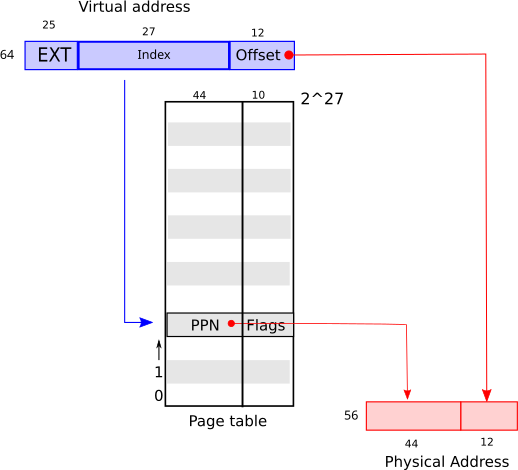
\includegraphics[scale=0.5]{fig/riscv_address.pdf}
\caption{An abstract view of a flat page table mapping virtual to physical addresses.}
\label{fig:riscv_address}
\end{figure}

xv6++ uses RISC-V's Sv39 mode, which means that only the bottom 39 bits
of a 64-bit virtual address are used; the top 25 bits are not used. In
this Sv39 configuration, a RISC-V page table is logically an array of
$2^{27}$ (134,217,728) \indextext{page table entries (PTEs)}. Each PTE
contains a 44-bit physical page number (PPN) and some flags.

The paging hardware translates a virtual address by using the top 27
bits of the 39 bits to index into the page table to find a PTE, and
making a 56-bit physical address whose top 44 bits come from the PPN in
the PTE and whose bottom 12 bits are copied from the original virtual
address. Figure~\ref{fig:riscv_address} shows this process with a
logical view of the page table as a simple array of PTEs (the RISC-V
page table is actually a tree; see Figure~\ref{fig:riscv_pagetable} for
a fuller story).

A page table gives the operating system control over virtual-to-physical
address translations at the granularity of aligned chunks of 4096
($2^{12}$) bytes. Such a chunk is called a \indextext{page}.

\begin{figure}[t]
\center
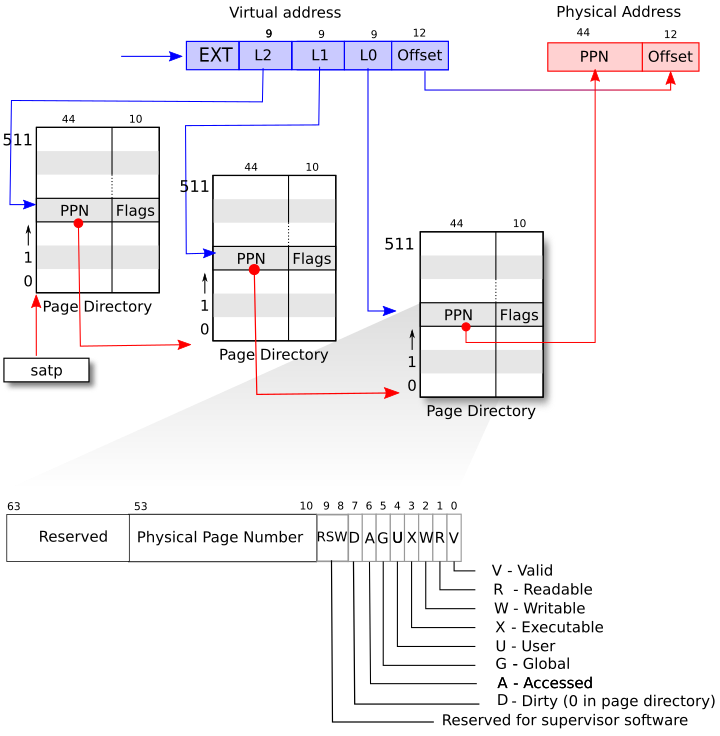
\includegraphics[scale=0.5]{fig/riscv_pagetable.pdf}
\caption{RISC-V address translation details.}
\label{fig:riscv_pagetable}
\end{figure}

RISC-V's design leaves room for expansion of both virtual and physical
addresses. If more virtual address space is needed, RISC-V supports an
Sv48 mode, with 48-bit virtual addresses~\cite{riscv:priv}. Physical
addresses also have room for growth: there is room in the PTE format for
the physical page number to grow by another 10 bits. The designers of
RISC-V chose address sizes based on technology predictions. $2^{48}$
bytes is 262,144 GB, a much larger user virtual address space than any
application is likely to use today. $2^{56}$ bytes of physical address
space is 65,536 terabytes, much more RAM than any computer can
currently be equipped with.

As Figure~\ref{fig:riscv_pagetable} shows, a RISC-V CPU page table is
stored in physical memory as a three-level tree. The root of the tree is
a 4096-byte page-table page that contains 512 PTEs, which contain the
physical addresses for page-table pages in the next level of the tree.
Each of those pages contains 512 PTEs for the final level in the tree.
The paging hardware uses the top 9 bits of the 27 bits to select a PTE
in the root page-table page, the middle 9 bits to select a PTE in a
page-table page in the next level of the tree, and the bottom 9 bits to
select the final PTE. (In Sv48 RISC-V a page table has four levels, and
bits 39 through 47 of a virtual address index into the top-level.)

If any of the three PTEs required to translate an address is not present,
the paging hardware raises a \indextext{page-fault exception}, leaving it
up to the kernel to handle the page fault (see Chapters~\ref{CH:TRAP}
and~\ref{CH:PGFAULTS}).

The three-level structure of Figure~\ref{fig:riscv_pagetable} allows a
memory-efficient way of recording PTEs, compared to the single-level
design of Figure~\ref{fig:riscv_address}. In the common case in which
large ranges of virtual addresses have no mappings, the three-level
structure can omit entire page directories. For example, if an
application uses only a few pages starting at address zero, then the
entries 1 through 511 of the top-level page directory are invalid, and
the kernel doesn't have to allocate pages for those 511 intermediate
page directories. Furthermore, the kernel also doesn't have to allocate
pages for the bottom-level page directories for those 511 intermediate
page directories. So, in this example, the three-level design saves 511
pages for intermediate page directories and $511\times512$ pages for
bottom-level page directories.

Although a CPU walks the three-level structure in hardware as part of
executing a load or store instruction, a potential downside of three
levels is that the CPU must load three PTEs from memory to perform the
translation of the virtual address in the load/store instruction to a
physical address. To avoid the cost of loading PTEs from physical
memory, a RISC-V CPU caches page table entries in a
\indextext{Translation Look-aside Buffer (TLB)}.

Each PTE contains flag bits that tell the paging hardware how the
associated virtual address is allowed to be used.
\indexcode{PTE_V} indicates whether the PTE is present: if it is not
set, a reference to the page causes a page fault (i.e., is not allowed).
\indexcode{PTE_R} controls whether instructions are allowed to read the page.
\indexcode{PTE_W} controls whether instructions are allowed to write the page.
\indexcode{PTE_X} controls whether the CPU may interpret the content of the
page as instructions and execute them.
\indexcode{PTE_U} controls whether instructions in user mode are allowed to
access the page; if \indexcode{PTE_U} is not set, the PTE can be used only in
supervisor mode. Figure~\ref{fig:riscv_pagetable} shows where the flag bits sit
in a PTE.

The flags and related paging definitions are in \texttt{kernel/riscv.h}.

To tell a CPU to use a page table, the kernel must write the physical
address of the root page-table page into the \texttt{satp} register
(see \texttt{kernel/riscv.h}). A CPU will translate all addresses
generated by subsequent instructions using the page table pointed to by
its \texttt{satp}. Each CPU has its own \texttt{satp} so that different
CPUs can run different processes, each with a private address space
described by its own page table.

From the kernel's point of view, a page table is data stored in memory,
and the kernel creates and modifies page tables using code much like you
might see for any tree-shaped data structure.

A few notes about terms used in this book. \textit{Physical memory}
refers to storage cells in RAM. A byte of physical memory has an
address, called a \textit{physical address}. Instructions that
dereference addresses (such as loads, stores, jumps, and function calls)
use only virtual addresses, which the paging hardware translates to
physical addresses, and then sends to the RAM hardware to read or write
storage.

An \textit{address space} is the set of virtual addresses that are valid in
a given page table; each xv6++ process has a separate user address space,
and the xv6++ kernel has its own address space as well. \textit{User memory}
refers to a process's user address space plus the physical memory that
the page table allows the process to access. \textit{Virtual memory} refers
to the ideas and techniques associated with managing page tables and using
them to achieve goals such as isolation.

\begin{figure}[h]
\centering
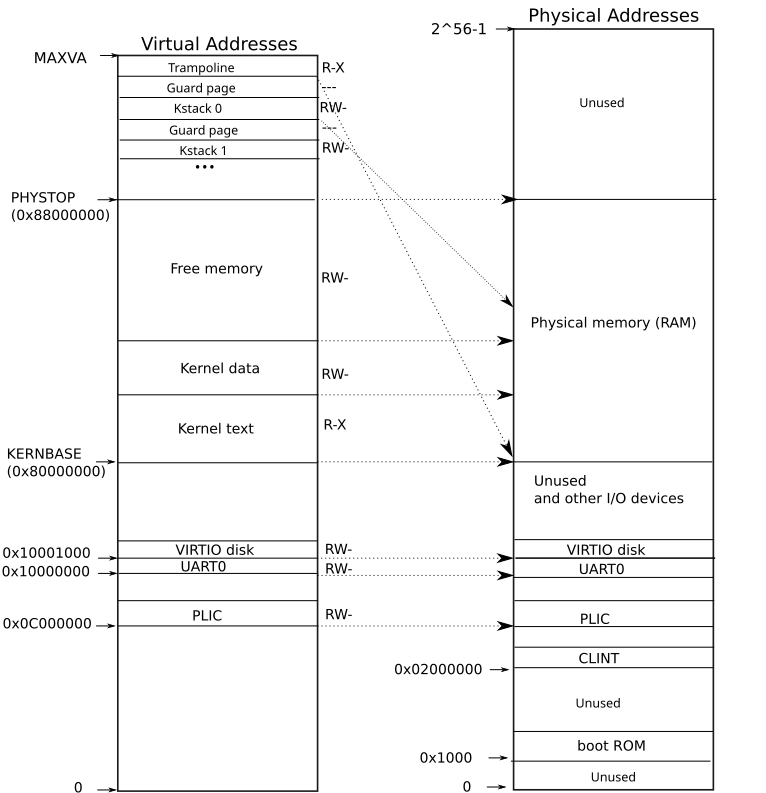
\includegraphics[scale=0.65]{fig/xv6_layout.pdf}
\caption{On the left, xv6++'s kernel virtual address space.
{\sf \small{RWX}} refer to PTE read, write, and execute permissions.
On the right, the RISC-V physical address space that xv6++ expects to see.}
\label{fig:xv6_layout}
\end{figure}

%%
\section{Kernel address space}
%%
When it starts, xv6++ creates a single page table describing the kernel's
address space. The kernel configures the layout of its address space to give
itself access to physical memory and various hardware resources at predictable
virtual addresses. Figure~\ref{fig:xv6_layout} shows how this layout maps
kernel virtual addresses to physical addresses.

The constants for xv6++'s physical and kernel memory layout are in
\texttt{kernel/memlayout.h}.

QEMU simulates a computer that includes RAM (physical memory) starting at
physical address \texttt{0x80000000} and continuing through at least
\texttt{0x88000000}, which xv6++ calls \texttt{PHYSTOP} (see
\texttt{kernel/memlayout.h}). The QEMU simulation also includes I/O
devices such as a disk interface. QEMU exposes the device interfaces to
software as \indextext{memory-mapped} control registers that sit below
\texttt{0x80000000} in the physical address space. The kernel can
interact with the devices by reading/writing these special physical
addresses; such reads and writes communicate with device hardware rather
than with RAM. Chapter~\ref{CH:TRAP} explains how xv6++ interacts with
devices.

The kernel maps all physical RAM and device registers at virtual
addresses equal to the physical addresses. This is called ``direct
mapping,'' and allows the kernel to read or write physical address $x$
simply by loading or storing to virtual address $x$.

The kernel code itself is located at \lstinline{KERNBASE=0x80000000} in
both the virtual address space and in physical memory (see
\texttt{kernel/memlayout.h}).

There are a couple of kernel virtual addresses that aren't direct-mapped:

\begin{itemize}

\item The trampoline page. It is mapped at the top of the virtual address
  space; user page tables have this same mapping. Chapter~\ref{CH:TRAP}
  discusses the role of the trampoline page, but we see here an
  interesting use case of page tables: a physical page (holding the
  trampoline code) is mapped twice in the virtual address space of the
  kernel: once at the top of the virtual address space and once with a
  direct mapping.

\item The kernel stack pages. Each process has its own kernel stack,
  which is mapped at a high kernel virtual address so that below it xv6++
  can leave an unmapped \indextext{guard page}. The guard page's PTE is
  invalid (i.e., \lstinline{PTE_V} is not set), so that if the kernel
  overflows a kernel stack, it will likely cause a page fault and the
  kernel will panic. Without a guard page an overflowing stack would
  overwrite other kernel memory, resulting in incorrect operation. A
  panic crash is preferable.

\end{itemize}

While the kernel uses its stacks via the high-memory mappings, each is
also accessible to the kernel through a direct-mapped address. An
alternate design might have just the direct mapping, and use the stacks
at the direct-mapped address. In that arrangement, however, providing
guard pages would involve unmapping virtual addresses that would
otherwise refer to physical memory, which would then be hard to use.

The kernel maps the pages for the trampoline and the kernel text with the
permissions \lstinline{PTE_R} and \lstinline{PTE_X}, but not
\lstinline{PTE_W}. The kernel maps other pages with the permissions
\lstinline{PTE_R} and \lstinline{PTE_W}, but not \lstinline{PTE_X}. The
mappings for the guard pages are invalid.

The purpose of these restricted permissions is to help catch kernel bugs
that access pages in unexpected ways, for example if kernel code
accidentally tried to write over kernel instructions.

xv6++ creates a single kernel page table, used by all CPUs when they
execute in the kernel. xv6++ does not modify the kernel page table after
initially creating it.

%%
\section{Code: creating an address space}
%%

Before proceeding, skim the virtual memory implementation (see
\texttt{kernel/virtual\_memory.h} and its corresponding \texttt{.cpp}).

In xv6++, the code for manipulating address spaces and page tables lives
in the \texttt{virtual\_memory} module (see \texttt{kernel/virtual\_memory.h}).
The central data structure is \lstinline{pagetable_t}, which is a pointer
to a RISC-V root page-table page (see \texttt{kernel/riscv.h}). A
\lstinline{pagetable_t} may be either the kernel page table, or one of
the per-process page tables.

Key functions include:
\begin{itemize}
\item \lstinline{virtual_memory::walk()}, which finds the PTE for a virtual address.
\item \lstinline{virtual_memory::mappages()}, which installs PTEs for new mappings.
\item \lstinline{virtual_memory::copyin()}, \lstinline{copyout()}, and \lstinline{copyinstr()},
      which copy data between kernel memory and user virtual addresses (see \texttt{kernel/virtual\_memory.h}).
\end{itemize}

Early in the boot sequence, the kernel initializes the kernel page table
with \lstinline{virtual_memory::init()} (see \texttt{kernel/virtual\_memory.h}).
This occurs before paging is enabled on the RISC-V, so addresses refer
directly to physical memory.

During initialization, xv6++ allocates a page of physical memory to hold
the root page-table page, and then installs the translations the kernel
needs. These translations include the kernel's instructions and data,
physical memory up to \lstinline{PHYSTOP}, and memory ranges that are
actually devices (see \texttt{kernel/memlayout.h}).

xv6++ also allocates a kernel stack for each process and maps each stack
at a high virtual address, leaving room for invalid stack-guard pages.
This work is performed by \lstinline{process_manager::mapstacks()}
(see \texttt{kernel/process\_manager.h} and \texttt{kernel/memlayout.h}).

The helper that installs kernel mappings ultimately calls
\lstinline{virtual_memory::mappages()}, which installs mappings into a
page table for a range of virtual addresses to a corresponding range of
physical addresses. It does this separately for each virtual address in
the range, at page intervals. For each virtual address to be mapped,
\lstinline{mappages} calls \lstinline{walk} to find the address of the PTE
for that address. It then initializes the PTE to hold the relevant
physical page number, the desired permissions (\lstinline{PTE_W},
\lstinline{PTE_X}, and/or \lstinline{PTE_R}), and \lstinline{PTE_V} to mark
the PTE as valid (see \texttt{kernel/riscv.h}).

\lstinline{virtual_memory::walk()} mimics the RISC-V paging hardware as it
looks up the PTE for a virtual address (see Figure~\ref{fig:riscv_pagetable}).
\lstinline{walk} descends the page table tree one level at a time, using each
level's 9 bits of virtual address to index into the relevant page-table page.
At each level it finds either the PTE of the next level's page-table page, or
the PTE of the final page. If a PTE in a first or second level page-table page
isn't valid, then the required page-table page hasn't yet been allocated; if the
\lstinline{alloc} argument is set, \lstinline{walk} allocates a new page-table page
and puts its physical address in the PTE. It returns the address of the PTE in the
lowest layer in the tree.

This code depends on physical memory being direct-mapped into the kernel
virtual address space. For example, as \lstinline{walk} descends levels of
the page table, it pulls the (physical) address of the next-level-down
page table from a PTE, and then uses that address as a virtual address to
fetch the PTE at the next level down.

On each CPU, xv6++ calls \lstinline{virtual_memory::inithart()} to install
the kernel page table (see \texttt{kernel/virtual\_memory.h}), placing the
physical address of the root page-table page into the CPU's \texttt{satp}
register (see \texttt{kernel/riscv.h}). After this the CPU translates
addresses using the kernel page table. The kernel continues to execute
correctly because the kernel page table is direct-mapped, so that
addresses refer to the same locations in RAM before and after this change.

Each RISC-V CPU caches page table entries in a
\indextext{Translation Look-aside Buffer (TLB)}, and when xv6++ changes a
page table, it must tell the CPU to invalidate corresponding cached TLB
entries. If it didn't, then at some point later the TLB might use an old
cached mapping, pointing to a physical page that in the meantime has been
allocated to another process, and as a result, a process might be able to
scribble on some other process's memory.

RISC-V has an instruction \indexcode{sfence.vma} that flushes the current
CPU's TLB (see \texttt{kernel/riscv.h}). xv6++ executes \lstinline{sfence.vma}
after updating \texttt{satp} and when switching between user and kernel
address spaces via the trampoline code.

It is also necessary to issue \texttt{sfence.vma} before changing \texttt{satp},
in order to wait for completion of all outstanding loads and stores. This wait
ensures that preceding updates to the page table have completed, and ensures
that preceding loads and stores use the old page table, not the new one.

\section{Physical memory allocation}

The kernel must allocate and free physical memory at run-time for page
tables, user memory, kernel stacks, and pipe buffers.

xv6++ uses the physical memory between the end of the kernel and
\indexcode{PHYSTOP} for run-time allocation. It allocates and frees whole
4096-byte pages at a time. It keeps track of which pages are free by
threading a linked list through the pages themselves. Allocation consists
of removing a page from the linked list; freeing consists of adding the
freed page to the list.

Please read the page allocator (see \texttt{kernel/page\_allocator.h} and its
corresponding \texttt{.cpp}).

%%
\section{Code: Physical memory allocator}
%%

In xv6++, the allocator is implemented by \lstinline{page_allocator}
(see \texttt{kernel/page\_allocator.h}). The allocator's data structure is a
\textit{free list} of physical memory pages that are available for allocation.
The free list is implemented as an \lstinline{intrusive_slist} (see
\texttt{kernel/intrusive\_slist.h}), meaning the ``next'' pointer is stored in
the free page itself.

The free list is protected by a \lstinline{spin_lock} (see \texttt{kernel/spin\_lock.h}).
For now, ignore the lock mechanics; Chapter~\ref{CH:LOCK} will examine locking
in detail.

The allocator initializes the free list to hold every page of physical RAM
between the end of the kernel and \lstinline{PHYSTOP}. xv6++ ought to determine
how much physical memory is available by parsing configuration information
provided by the hardware. Instead xv6++ assumes that the machine has 128 MB of RAM
(see \texttt{kernel/memlayout.h}).

The allocator sometimes treats addresses as integers in order to perform arithmetic
on them (for example, traversing all pages in a range), and sometimes uses addresses
as pointers to read and write memory (for example, manipulating the ``next'' pointer
stored in a free page). This dual use of addresses is the main reason that low-level
allocator code often contains type casts.

When freeing a page, xv6++ overwrites the freed memory with junk to help catch bugs
that use memory after freeing it (dangling references). Then it prepends the page to
the free list. Allocation removes and returns the first element in the free list
(see \texttt{kernel/page\_allocator.h}).

\section{Process address space}

Each process has its own page table, and when xv6++ switches between
processes, it also changes page tables. Figure~\ref{fig:processlayout}
shows a process's address space in more detail than
Figure~\ref{fig:xv6_layout}. A process's user address space starts at
zero and in principle ends at \texttt{MAXVA} (see \texttt{kernel/riscv.h}),
though in practice only a small fraction of this is mapped to physical
memory.

A process's address space consists of pages that contain the text of the
program (which xv6++ maps with the permissions \lstinline{PTE_R},
\lstinline{PTE_X}, and \lstinline{PTE_U}), pages that contain the
pre-initialized data of the program, a page for the stack, and pages for
the heap. xv6++ maps the data, stack, and heap with the permissions
\lstinline{PTE_R}, \lstinline{PTE_W}, and \lstinline{PTE_U}.

Using permissions within a user address space is a common technique to
harden a user process. If the text were mapped with \lstinline{PTE_W},
then a process could accidentally modify its own program; for example, a
programming error may cause the program to write to a null pointer,
modifying instructions at address 0, and then continue running, perhaps
creating more havoc. To detect such errors immediately, xv6++ maps the
text without \lstinline{PTE_W}; if a program accidentally attempts to
store to address 0, the hardware will refuse to execute the store and
raises a page fault (see Chapter~\ref{CH:TRAP}). The kernel then kills
the process and prints out an informative message so that the developer
can track down the problem.

Similarly, by mapping data without \lstinline{PTE_X}, a user program
cannot accidentally jump to an address in the program's data and start
executing at that address.

In the real world, hardening a process by setting permissions carefully
also aids in defending against security attacks. An adversary may feed
carefully-constructed input to a program (e.g., a Web server) that
triggers a bug in the program in the hope of turning that bug into an
exploit~\cite{aleph:smashing}. Setting permissions carefully and other
techniques, such as randomizing the layout of the user address space,
make such attacks harder.

The stack is a single page, and is shown with the initial contents as
created by the \lstinline{exec} system call. Strings containing the
command-line arguments, as well as an array of pointers to them, are at
the very top of the stack. Just under that are values that allow a
program to start at \lstinline{main} as if the function
\lstinline{main(argc, argv)} had just been called.

To detect a user stack overflowing the allocated stack memory, xv6++
places an inaccessible guard page right below the stack by clearing the
\lstinline{PTE_U} flag. If the user stack overflows and the process tries
to use an address below the stack, the hardware will generate a page-fault
exception because the guard page is inaccessible to a program running in
user mode. A real-world operating system might instead automatically
allocate more memory for the user stack when it overflows.

We see here a few nice examples of use of page tables. First, different
processes' page tables translate user addresses to different pages of
physical memory, so that each process has private user memory. Second,
each process sees its memory as having contiguous virtual addresses
starting at zero, while the process's physical memory can be
non-contiguous. Third, the kernel maps a page with trampoline code at the
top of the user address space (without \lstinline{PTE_U}), thus a single
page of physical memory shows up in all address spaces, but can be used
only by the kernel.

\begin{figure}[t]
\center
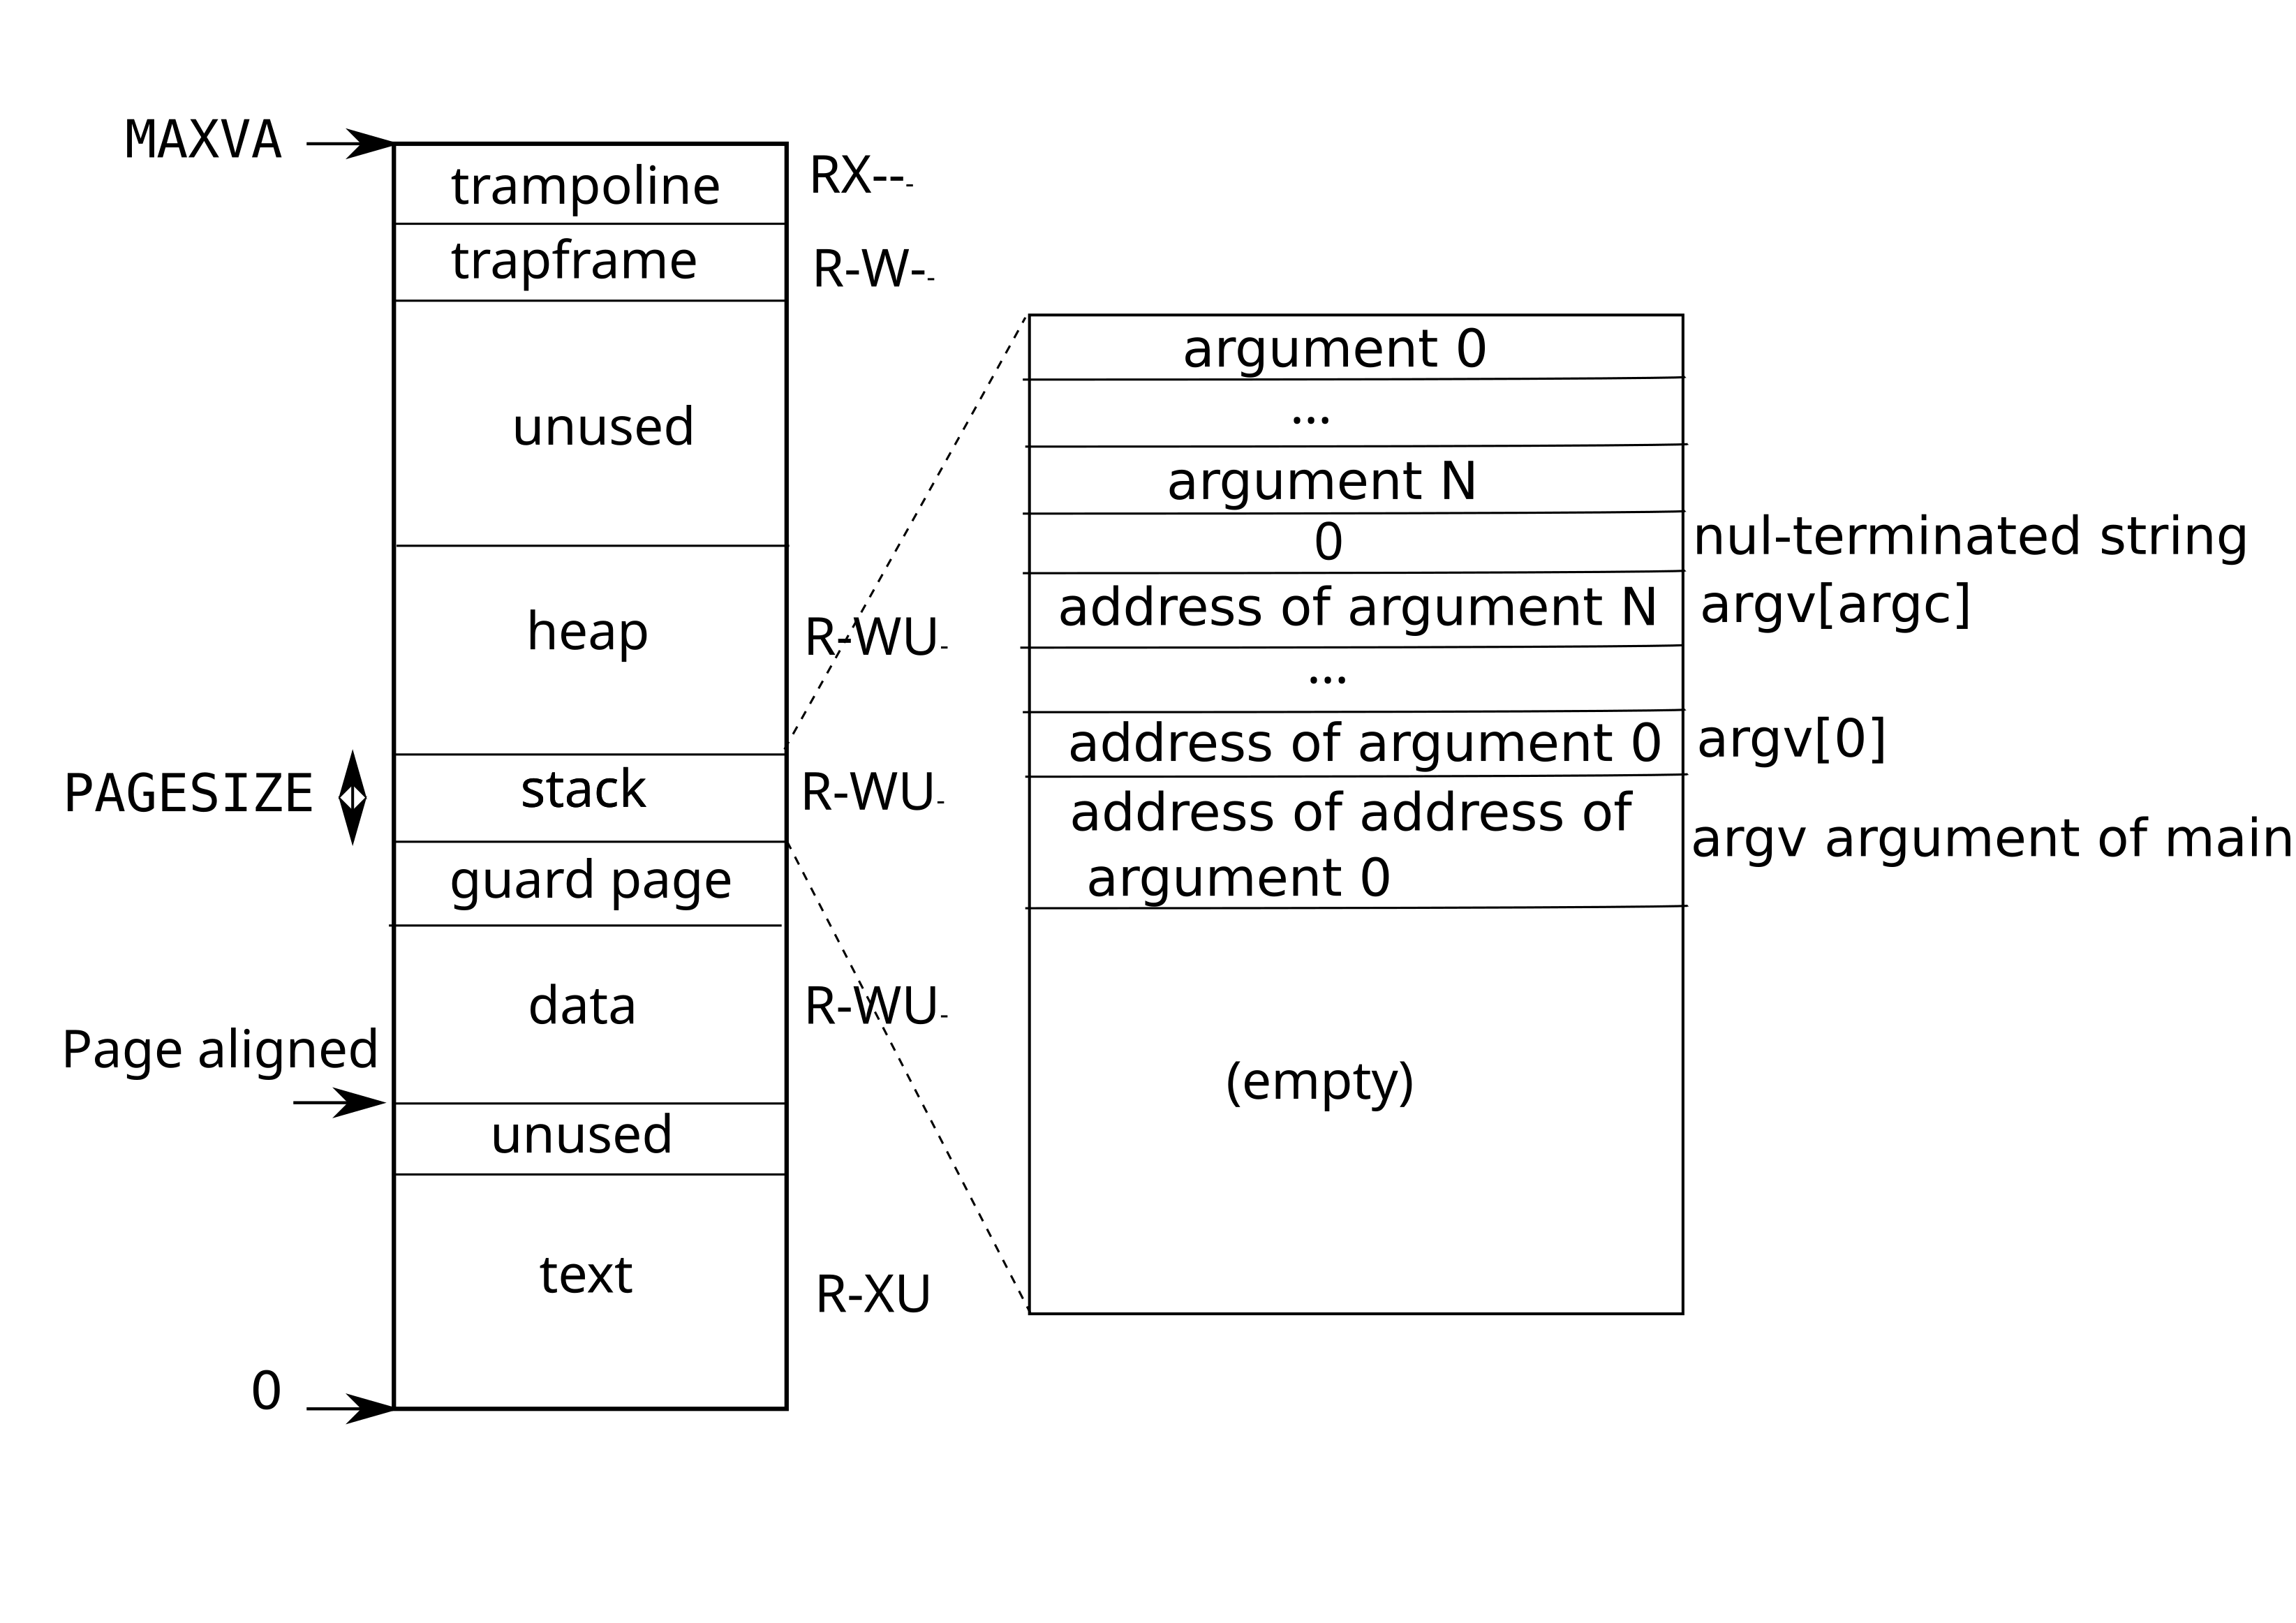
\includegraphics[scale=0.5]{fig/processlayout.png}
\caption{A process's user address space, with its initial stack.}
\label{fig:processlayout}
\end{figure}

%%
\section{Code: exec}
%%

Please read the process execution code (see \texttt{kernel/process.h}) and
the virtual memory code (see \texttt{kernel/virtual\_memory.h}),
especially the routines that allocate and map user pages.

\lstinline{exec} is a system call that replaces a process's user address
space with data read from a file, called a binary or executable file. A
binary is typically the output of the compiler and linker, and holds
machine instructions and program data.

In xv6++, \lstinline{process::exec()} implements \lstinline{exec} (see
\texttt{kernel/process.h}). It opens the named binary path using the
file system (see \texttt{kernel/file\_system.h}), then reads the ELF header.
xv6++ binaries are formatted in the widely-used \indextext{ELF format},
defined in \texttt{kernel/elf.h}. An ELF binary consists of an ELF header,
\indexcode{struct elfhdr}, followed by a sequence of program section headers,
\lstinline{struct proghdr} (see \texttt{kernel/elf.h}). Each \lstinline{proghdr}
describes a section of the application that must be loaded into memory; xv6
programs have two program section headers: one for instructions and one for data.

The first step is a quick check that the file probably contains an ELF
binary. An ELF binary starts with the four-byte ``magic number''
\lstinline{0x7F}, \lstinline{`E'}, \lstinline{`L'}, \lstinline{`F'},
or \indexcode{ELF_MAGIC} (see \texttt{kernel/elf.h}). If the ELF header has
the right magic number, xv6++ assumes that the binary is well-formed.

\lstinline{process::exec()} allocates a new page table with no user mappings,
allocates memory for each ELF segment, and loads each segment into memory.
Loading each segment relies on \lstinline{process::loadseg()} (see
\texttt{kernel/process.h}), and the virtual memory routines that translate
user virtual addresses to physical addresses (see \texttt{kernel/virtual\_memory.h}).

The program section header for \indexcode{/init}, the first user program created
with \lstinline{exec}, looks like this:
\begin{footnotesize}
\begin{verbatim}
# objdump -p user/_init

user/_init:     file format elf64-little

Program Header:
0x70000003 off    0x0000000000006bb0 vaddr 0x0000000000000000
                                       paddr 0x0000000000000000 align 2**0
         filesz 0x000000000000004a memsz 0x0000000000000000 flags r--
    LOAD off    0x0000000000001000 vaddr 0x0000000000000000
                                       paddr 0x0000000000000000 align 2**12
         filesz 0x0000000000001000 memsz 0x0000000000001000 flags r-x
    LOAD off    0x0000000000002000 vaddr 0x0000000000001000
                                       paddr 0x0000000000001000 align 2**12
         filesz 0x0000000000000010 memsz 0x0000000000000030 flags rw-
   STACK off    0x0000000000000000 vaddr 0x0000000000000000
                                       paddr 0x0000000000000000 align 2**4
         filesz 0x0000000000000000 memsz 0x0000000000000000 flags rw-
\end{verbatim}
\end{footnotesize}

We see that the text segment should be loaded at virtual address 0x0 in
memory (without write permissions) from content at offset 0x1000 in the
file. We also see that the data should be loaded at address 0x1000, which
is at a page boundary, and without executable permissions.

A program section header's \lstinline{filesz} may be less than the
\lstinline{memsz}, indicating that the gap between them should be filled
with zeroes (for C global variables) rather than read from the file. For
\lstinline{/init}, the data \lstinline{filesz} is 0x10 bytes and
\lstinline{memsz} is 0x30 bytes, and thus xv6++ allocates enough physical
memory to hold 0x30 bytes, but reads only 0x10 bytes from the file.

Next \lstinline{process::exec()} allocates and initializes the user stack.
It allocates just one stack page (see \texttt{kernel/param.h} where
\lstinline{USERSTACK} is defined). It copies the argument strings to the
top of the stack one at a time, recording the pointers to them in an array
that will become \lstinline{argv}. It places a null pointer at the end of
what will be the \lstinline{argv} list passed to \lstinline{main}. The values
for \lstinline{argc} and \lstinline{argv} are passed to \lstinline{main}
through the system-call return path: \lstinline{argc} is passed via the
system call return value (in register \texttt{a0}), and \lstinline{argv} is
passed through register \texttt{a1} (see \texttt{kernel/riscv.h} for calling
conventions and trapframe layout).

\lstinline{process::exec()} places an inaccessible page just below the
stack page, so that programs that try to use more than one page will fault.
This inaccessible page also allows \lstinline{exec} to deal with arguments
that are too large; in that situation, the \lstinline{virtual_memory::copyout()}
function used to copy arguments to the stack will notice that the destination
page is not accessible, and will return -1 (see \texttt{kernel/virtual\_memory.h}).

During the preparation of the new memory image, if \lstinline{exec} detects an
error like an invalid program segment, it frees the new image and returns -1.
It must wait to free the old image until it is sure that the system call will
succeed: if the old image is gone, the system call cannot return -1 to it.

The \lstinline{exec} system call loads bytes from the ELF file into memory at
addresses specified by the ELF file. Users can place whatever addresses they
want into an ELF file. Thus \lstinline{exec} is risky, because the addresses
in the ELF file may refer to kernel memory, accidentally or on purpose. The
consequences for an unwary kernel could range from a crash to a malicious
subversion of the kernel's isolation mechanisms (i.e., a security exploit).
xv6++ performs a number of checks to avoid these risks. For example,
\lstinline{if(ph.vaddr + ph.memsz < ph.vaddr)} checks whether the sum overflows
a 64-bit integer.

In the RISC-V version of xv6++ this kind of attack cannot directly overwrite the
kernel, because the kernel has its own separate page table; segments load into
the process's page table, not the kernel's page table.

It is easy for a kernel developer to omit a crucial check, and real-world
kernels have a long history of missing checks whose absence can be exploited
by user programs to obtain kernel privileges. It is likely that xv6++ doesn't
do a complete job of validating user-level data supplied to the kernel, which
a malicious user program might be able to exploit to circumvent xv6++'s isolation.

%%
\section{Real world}
%%

Like most operating systems, xv6++ uses the paging hardware for memory
protection and mapping. Most operating systems make far more sophisticated
use of paging than xv6++ by combining paging and page-fault exceptions,
which we will discuss in Chapter~\ref{CH:TRAP}.

xv6++ is simplified by the kernel's use of a direct map between virtual and
physical addresses, and by its assumption that there is physical RAM at
address 0x80000000, where the kernel expects to be loaded (see
\texttt{kernel/memlayout.h}). This works with QEMU, but on real hardware it
turns out to be a bad idea; real hardware places RAM and devices at
unpredictable physical addresses, so that (for example) there might be no RAM
at 0x80000000, where xv6++ expects to store the kernel. More serious kernel
designs exploit the page table to turn arbitrary hardware physical memory
layouts into predictable kernel virtual address layouts.

RISC-V supports protection at the level of physical addresses, but xv6++ doesn't
use that feature.

On machines with lots of memory it might make sense to use RISC-V's support for
``super pages.'' Small pages make sense when physical memory is small, to allow
allocation and page-out to disk with fine granularity. For example, if a program
uses only 8 kilobytes of memory, giving it a whole 4-megabyte super-page of
physical memory is wasteful. Larger pages make sense on machines with lots of RAM,
and may reduce overhead for page-table manipulation.

To avoid having to flush the complete TLB when changing page tables, RISC-V CPUs
may support address space identifiers (ASIDs)~\cite{riscv:priv}. The kernel can
then flush just the TLB entries for a particular address space. xv6++ does not
use this feature.

The xv6++ kernel's lack of a \texttt{malloc}-like allocator that can provide
memory for small objects prevents the kernel from using sophisticated data
structures that would require dynamic allocation. A more elaborate kernel would
likely allocate many different sizes of small blocks, rather than (as in xv6++)
just 4096-byte blocks; a real kernel allocator would need to handle small
allocations as well as large ones.

Memory allocation is a perennial hot topic, the basic problems being efficient
use of limited memory and preparing for unknown future requests~\cite{knuth}.
Today people care more about speed than space efficiency.

%%
\section{Exercises}
%%

\begin{enumerate}

\item Parse RISC-V's device tree to find the amount of physical memory the computer has.

\item The functions \texttt{copyin} and \texttt{copyinstr} walk the user page table in software
  (see \texttt{kernel/virtual\_memory.h}). Set up the kernel page table so that the kernel has the
  user program mapped, and \texttt{copyin} and \texttt{copyinstr} can use \texttt{memcpy} to copy
  system call arguments into kernel space, relying on the hardware to do the page table walk.

\item Modify xv6++ to use super pages for the kernel.

\item Unix implementations of \lstinline{exec} traditionally include special handling for shell scripts.
If the file to execute begins with the text \lstinline{#!}, then the first line is taken to be a program
to run to interpret the file. For example, if \lstinline{exec} is called to run \lstinline{myprog}
\lstinline{arg1} and \lstinline{myprog}'s first line is \lstinline{#!/interp}, then \lstinline{exec}
runs \lstinline{/interp} with command line \lstinline{/interp} \lstinline{myprog} \lstinline{arg1}.
Implement support for this convention in xv6++.

\item Implement address space layout randomization for the kernel.

\end{enumerate}
